\documentclass[conference]{IEEEtran}

% use natbib for author-year citations
\usepackage[round]{natbib}
% \usepackage{subcaption}

\usepackage{graphicx}
% \usepackage{hyperref}
\usepackage[hidelinks]{hyperref}
\usepackage{amsmath}
\usepackage{amssymb}
\usepackage{booktabs}
% \usepackage{cite}
\usepackage{subcaption}

\title{(Blind) Multimodal Bot Detection on X}
\author{Hamza Rashid \\ McGill University \\ COMP 400}
\date{\today}

\begin{document}

\maketitle

\begin{abstract}
This research investigates multimodal bot
detection methods on X, in a setting where
the labels are not known a priori, and graph data is not available.
We present a comprehensive evaluation of bot detection 
by benchmarking classical machine-learning baselines
and feature engineering techniques, 
and later develop deep multimodal architectures. 
Our work begins with conventional classifiers---a random forest 
on text, temporal, and topic-distribution features, 
yielding moderate baseline performance. 
We next investigate how humans and bots differ in their 
temporal posting behaviour, finding little
distinction except for outliers. As
feature engineering approaches are easily deceived by sophisticated bots, 
we move on to multimodal architectures with an emphasis on DNA-inspired 
behaviour modeling. For this, we embed the user description with 
TwHIN-BERT and model posting behavior with two DNA formulations, 
one that captures content across posts, and another capturing inter-post times.
We find that CNN embeddings of inter-post time DNA may capture deep
patterns in time series data that conventional methods miss.
We investigate three methods for processing the modalities 
and final fusion; a GMU (gated multimodal unit), 
a cross-attention mechanism, and a sparsely gated MOE (mixture-of-experts)
with a self-attention fusion layer and a convolution learned on attention weights
that addresses manipulated features. 
We find that the MOE performs best, and gather counter-intuitive results along the way. 
Namely, the MOE is the smallest of our multimodal models, and does not require any treatment
of the class imbalance found in bot detection datasets. 
More broadly, we find that a multimodal approach to bot detection 
improves robustness against sophisticated bots, and that a MOE
architecture helps in addressing the diversity of user communities on X. 
\end{abstract}

\section{Introduction}
Social media platforms like X (formerly Twitter) have 
enabled unprecedented global connectivity. 
As an open platform is vulnerabe, X is fertile ground for malicious content,
often originating from automated accounts—bots—that manipulate discourse, spread misinformation, or artificially amplify content. 
Detecting and mitigating such bot activities remains a challenging yet essential task for preserving authentic online interactions.

Traditional approaches to bot detection typically rely on supervised classification methods trained on manually labeled datasets. Yet, in real-world scenarios, labeled data are often scarce, outdated, or non-representative of the evolving behaviors exhibited by sophisticated bots. Consequently, there is a pressing need for detection methods that generalize beyond known bot patterns, especially in contexts where labeled data is not readily available.

In this report, we address this challenge by evaluating a range of bot detection strategies, beginning with classical machine-learning techniques enhanced by extensive feature engineering. We initially employ a random forest classifier incorporating textual features, temporal posting patterns, and inferred topic distributions, achieving moderate baseline performance. Our analysis reveals that traditional temporal features often fail to effectively distinguish sophisticated bots from genuine users, underscoring the limitations of classical approaches.

Building on these insights, we introduce deep multimodal architectures designed to exploit richer behavioral patterns. Inspired by the concept of digital DNA, our method integrates user descriptions embedded via TwHIN-BERT and models posting behavior through two distinct DNA formulations: one capturing the content across posts and another encoding inter-post timing patterns. 
In addition to the known efficacy of content DNA \citep{ilias2023multimodal}, our experiments demonstrate that CNNs applied to temporal-DNA-generated images effectively uncover nuanced behavioral patterns overlooked by conventional methods. As most of the frontier literature 
overlooks temporal bevahiour, this result signifies that it could be worth further investigation.

We further explore several fusion techniques to integrate multimodal signals, including gated multimodal units (GMUs), cross-attention mechanisms, and a novel application of a sparsely gated mixture-of-experts (MOE) \citep{shazeer2017outrageously} architecture. 
Our results highlight the MOE model's superior performance and efficiency, notably without necessitating explicit strategies to address class imbalance. Overall, our research emphasizes the 
robustness of multimodal approaches and illustrates the potential of MOE architectures to adapt effectively to the diverse user communities found on X.


\section{Dataset and Experimental Setup}

Our experiments were conducted within the "Bot Or Not" (B.O.N.) competitive infrastructure, designed specifically for assessing bot detection strategies in realistic social media scenarios. 
As it is currently in the development phase, the conditions outlined in this report are subject to change in future versions.
This environment featured interactions between bot and detector teams, simulating genuine activities on the X platform. 
The primary goal was to evaluate the effectiveness of detection methodologies under conditions closely resembling live social media dynamics.

\subsection{Data Collection and Characteristics}

The dataset comprised real posts gathered from the X API across multiple collection sessions, 
each lasting the same duration but occurring on different days. For each session, posts were 
initially collected based on predefined sets of topical keywords relevant to that session. 
After gathering initial posts, users flagged as obvious bots were removed, and the dataset was 
expanded by including all additional posts from the remaining users within the session period. 

The preliminary data collection process can summarized as follows:
\begin{itemize}
    \item Text-only Posts: Posts containing images, videos, or memes were excluded.

    \item Static Metadata: Dynamic metadata such as likes, comments, and follower counts were excluded to maintain consistency and simplicity.

    \item Anonymized Links and Mentions: Hyperlinks were standardized to ``https://t.co/twitter\_link'', and user mentions were anonymized to ``@mention'' to prevent easy verification of authenticity.
    
    \item Activity Thresholds: Each included user produced between 10 and 100 posts during the session period, ensuring active participation.
\end{itemize}

% Instruction: comment on how the above limits the scope of our research, e.g., no graph data to work with like following/follwed by, likes, etc
Datasets were structured into two main JSON formats:
\begin{itemize}
    \item Posts Dataset: Included text content, timestamp, unique post ID, author ID, and language.
    
    \item Users Dataset: Contained user-specific metadata, including user ID, username, display name, profile description, location, tweet count, and a calculated activity-based z-score.
\end{itemize}

\subsection{Session Structure}

Sessions were divided into multiple sequential sub-sessions to mimic the real-time flow of social media feeds, gradually introducing new posts to participants. Bot teams generated content incrementally across these sub-sessions, with the requirement to post between 10 and 100 posts per bot by session completion. Detector teams subsequently analyzed the fully compiled datasets post-session to identify bots, providing both binary verdicts and confidence scores for each account.

\subsection{Technical Setup}

Participant submissions (bot and detector code) were managed via public GitHub repositories cloned into Docker images deployed on EC2 instances, ensuring standardized computing resources and fair evaluation conditions. Submissions were required to execute fully within a one-hour timeframe, after which automated shutdown procedures terminated any ongoing processes.


\section{Methodology}

Our approach involved a systematic progression from classical machine learning methods to multimodal neural-based architectures, 
aimed at overcoming limitations observed at each stage. 
The lack of graph and user meta data limited the scope of our research.
We nonetheless explored methods that are capable of utilizing such features 
with minimal adjustments.
Our primary goal was to model user behaviour
from a variety of perspectives since nontrival bots manipulate features in at least one aspect 
(e.g., tweet content, posting times, or interactions such as retweets, likes, and follower and following relationships).
%  Instruction: in the below sub/subsub-sections, make the language a bit more formal; e.g, 'statistics' instead of 'stats', etc and find titles more formal than 'what went right' and 'what went wrong'
\subsection{Baseline - Random Forest}
Our baseline method involved training a Random Forest classifier using various 
handcrafted and learned features from user posts. We organized our experiments across 
multiple data collection sessions to assess how well feature-based models generalize 
across batches of social media activity. The sub-approaches below correspond to progressively 
enriched feature sets tested on different sessions. The primary motivation
for employing a random forest is that it enables rapid feature exporation due to its
flexibility (allows multiple data types in its feature set), and its proven efficacy in bot detection,
most notably in Botometer \citep{davis2016botornot}.

\subsubsection{Session 11 – Embeddings + LDA}
We began with a straightforward approach combining sentence-level embeddings with LDA (Latent Dirichlet Allocation)-based topic distributions. 
Each user’s posts were aggregated into a single document, from which features were extracted.

Implementation Summary:
\begin{itemize}
    \item Text Cleaning: URLs, mentions, and hashtags were anonymized. Tokenization, lemmatization, and stopword filtering were performed using spaCy.
    
    \item Embedding: Posts were embedded using all-MiniLM-L6-v2 from SentenceTransformers.
    
    \item Topic Modeling: CountVectorizer was used for bag-of-words representations, followed by LDA with 10 topics.
    
    \item Sentence embeddings (384-dim) were concatenated with LDA topic distributions.
    
    \item Classifier: A balanced Random Forest with 100 trees was trained and evaluated using stratified 80/20 train/test splits.
\end{itemize}

Result:
The model exbihibted low confidence and marked all samples as negatives. This likely owes
to its reliance on predefined topics, which vary across sessions, resulting in sparse vectors 
on unseen data.

Limitations:
\begin{itemize}
    \item Did not use individual tweets as independent samples, thereby lacking granulrity.
    
    \item Static topic modeling limited generalization to new sessions.
\end{itemize}

\subsubsection{Session 12 – Mean Embedding + BERTopic + Temporal Stats}
In this session, we shifted to using per-tweet embeddings and adopted BERTopic for more dynamic topic modeling. Additional temporal statistics were introduced to capture behavioral rhythms.

Implementation Summary:
\begin{itemize}
    \item Tweet-Level Processing: Individual tweets were embedded and clustered into topics using BERTopic with HDBSCAN.
    
    \item Aggregation: User-level features were computed via:
    \begin{itemize}
        \item  Mean of sentence embeddings
        
        \item Normalized topic distribution (padded to 361 dimensions)
    \end{itemize}
    
    \item Temporal features: mean and standard deviation of post timestamps
    
    \item Static features: Post count
    
    \item Classifier: The same Random Forest model from Session 11 was applied.
\end{itemize}


Result:
The use of dynamic topic modeling and behavioral signals significantly improved classification performance. Bot recall improved due to BERTopic's unsupervised generalization across sessions.

Limitations:
\begin{itemize}
    \item Topic dimension padding was static and could introduce noise.
    
    \item Temporal features were still limited to coarse statistics.
\end{itemize}

\subsubsection{Session 13 – Enhanced Temporal Behavior Modeling}
Session 13 introduced a novel temporal feature: duplicate post timestamps within bucketed time intervals, designed to capture artificial timing artifacts used by bots.

Implementation Summary:
\begin{itemize}
    \item Building on Session 12, we added:
    
    \item Inter-post Interval Statistics: Mean and standard deviation of time gaps between posts.
    
    \item Bucketed Duplicate Counts: Timestamps were partitioned into 10 intra- and inter-chronologically-ordered buckets, and duplicate post counts were computed per bucket.
    
    \item Features Used: Combined embeddings, topic distributions, post frequency, inter-post intervals, and bucketed duplicates.
\end{itemize}
    
Result:
This was the strongest-performing Random Forest baseline. The bucketed duplicates provided a clear signal in identifying bots with repeated behavior patterns or scheduled posts.

Limitations:
\begin{itemize}
    \item Still relied heavily on session-specific BERTopic clusters.
    
    \item Lacked explicit modeling of inter-feature dependencies (e.g., topic-time correlations).
\end{itemize}

\subsubsection{Session 14 – Topic Statistics + Temporal Entropy + Intra-Topic Similarity}
This final Random Forest setup expanded feature engineering to include statistical, temporal, and semantic regularities observed in bot behavior. 
The design aimed to encode not just what a user posts, but also how, and when, consistently.

Implementation Summary:
\begin{itemize}
    \item Refined Preprocessing: Hashtags were partially preserved (\texttt{\#arena $\rightarrow$ <HashtagMention:arena>}), preserving topic cues often used by bots.
    
    \item Normalized Embeddings: Sentence embeddings (MiniLM-L6-v2) were explicitly normalized to prevent variance from dominating downstream signals.
    
    \item Topic Modeling: BERTopic + HDBSCAN, followed by:
    \begin{itemize}
        \item Topic Histogram (topic mention counts across topics)
        \item Summary Statistics: Mean, variance, std, entropy, and dominance ratio across topic indices.
    \end{itemize}
    
    \item Temporal Signals:
    \begin{itemize}
        \item  Mean, std, and variance of time between posts.
        \item Bucketed duplicate timestamps (tolerance-aware) to flag spam bursts
    \end{itemize}
    
    \item Intra-topic Semantic Consistency:
    \begin{itemize}
        \item Mean, median, and std of pairwise cosine similarities across tweets within each user-topic group.
    \end{itemize}
\end{itemize}

Result:
In session 14, the bots became more difficult to distinguish. That is,
this model outperformed its predecessor under the same training conditions 
when applied to the previous session, but performed worse on the latest.
% Insert final accuracy, precision, recall, F1 scores here.
% Note if performance improved significantly over earlier sessions.
% Mention if any new features proved particularly important (e.g., topic entropy, similarity mean).

Limitations:
\begin{itemize}
    \item Feature dimensionality increased significantly, potentially stressing interpretability.
    
    \item BERTopic remains sensitive to session-specific clustering variance.
\end{itemize}

\subsection{Summary and Reflection on Random Forest Baseline}
Our progression through four sessions using Random Forest classifiers illustrates the evolving challenge of distinguishing bots from humans on X through feature engineering alone.

What Went Right:
\begin{itemize}
    \item Rich Feature Design: Session 14 demonstrates that carefully designed user-level features (temporal, semantic, topical) can yield strong performance using classical models despite evolving bots.
    
    \item Dynamic Topic Modeling: Transitioning from static LDA to BERTopic+HDBSCAN enabled models to better capture cross-session topical drift.
    
    \item Behavioral Signals Help: Features such as inter-post intervals and intra-topic semantic consistency offered important signals for detecting scripted or bursty behavior patterns.
\end{itemize}

What Went Wrong:
\begin{itemize}
    \item Sensitivity to Session Artifacts: A non-pretrained BERTopic model was applied to each session, 
    which likely created inconsistencies in how topic-features were interpreted by the classifier.
    
    \item Appropriateness of features: Despite being a universal approximator, Random Forest's are typically geared towards categorical features; introducing several related continuous features like embeddings can introduce noise.
    
    \item Limited Generalization: Although high accuracy may have been achieved on per-session splits, the performance likely degraded when faced with unseen session distributions or bot styles.
    
    \item Feature Brittleness: Despite capturing many dimensions, these features are often brittle against slight changes in bot strategies (e.g., using synonyms or reworded hashtags).
    
    \item Scalability Concerns: Computing transformer embeddings, pairwise similarities, multiple topic statistics, and padded histograms scales poorly for large user datasets.
\end{itemize}
While the Random Forest baseline allowed us to test many ideas rapidly, 
its limitations became evident in detecting sophisticated or adaptive bots (increasing complexity of feature engineering was needed to keep up with the bots), 
motivating the shift to multimodal methods whose underlying features and architecture 
can adapt to evolving behaviours on X. 

Before proceeding to our multimodal methods, we demonstrate the need
for more dynamic representations.



\subsection{Temporal Feature Analysis via KS Tests}
To assess the discriminative power of static temporal features, 
we computed inter-post interval distributions for each user and 
performed Kolmogorov--Smirnov (KS) tests against four theoretical 
models: exponential, normal, lognormal, and Weibull. Figures~\ref{fig:ks_exponential}-\ref{fig:ks_weibull} 
display the resulting KS statistic distributions for bots versus humans.
A lower KS value indicates a better fit to 
the assumed distribution, while a higher value 
implies greater deviation from the theoretical model. 
% The significant overlap indicates that these time-based summaries alone are insufficient, motivating the temporal-DNA in our multimodal architectures.

% To motivate our use of temporal-DNA in the multimodal architecture, we provide statistical 
% goodness-of-fit tests using the Kolmogorov–Smirnov (KS) statistic, showing little difference between humans and bots, 
% except for outliers. 
% For each user, we fit four different distributions---Exponential, Lognormal, Normal, 
% and Weibull—--to their inter-post gaps and computed the KS statistic between the 
% empirical and fitted distributions.
% A lower KS value indicates a better fit to 
% the assumed distribution, while a higher value 
% implies greater deviation from the theoretical model. 

\begin{figure}[htbp]
    \centering

    \begin{subfigure}[b]{0.48\linewidth}
        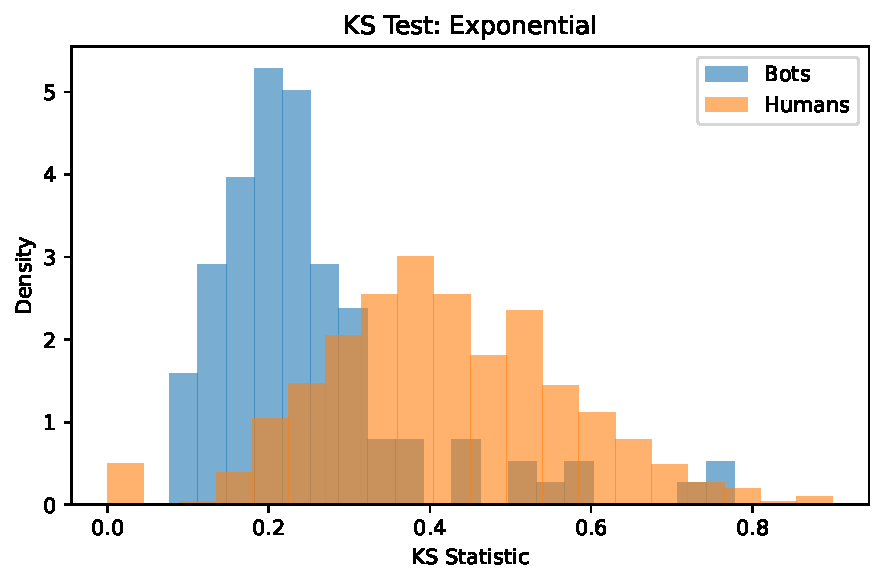
\includegraphics[width=\linewidth]{../figures/ks_exponential.pdf}
        \caption{Exponential model}
        \label{fig:ks_exponential}
    \end{subfigure}
    \hfill
    \begin{subfigure}[b]{0.48\linewidth}
        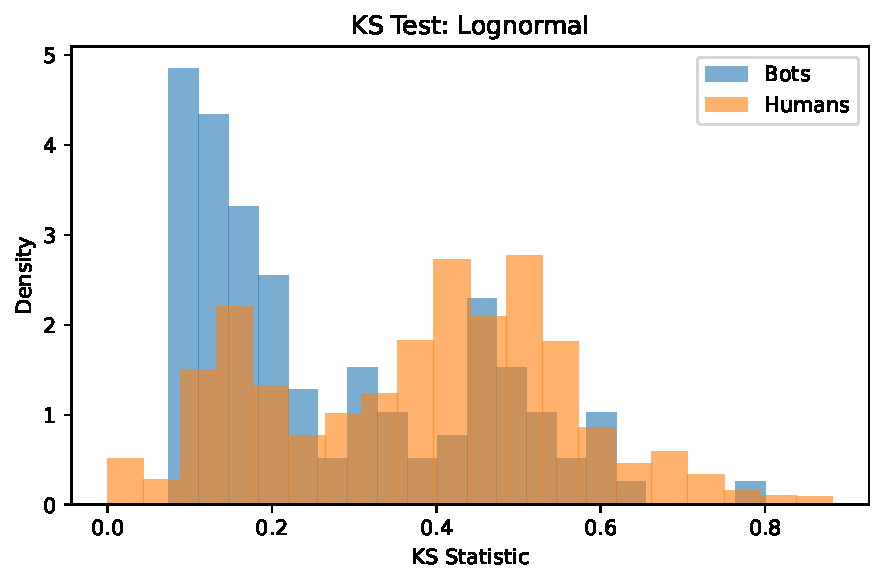
\includegraphics[width=\linewidth]{../figures/ks_lognormal.pdf}
        \caption{Lognormal model}
        \label{fig:ks_lognormal}
    \end{subfigure}

    \vspace{1em}

    \begin{subfigure}[b]{0.48\linewidth}
        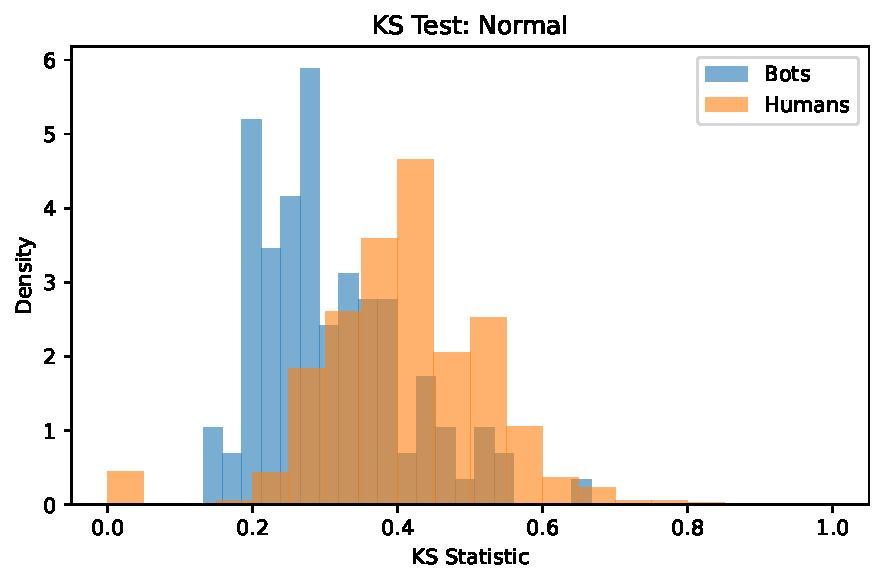
\includegraphics[width=\linewidth]{../figures/ks_normal.pdf}
        \caption{Normal model}
        \label{fig:ks_normal}
    \end{subfigure}
    \hfill
    \begin{subfigure}[b]{0.48\linewidth}
        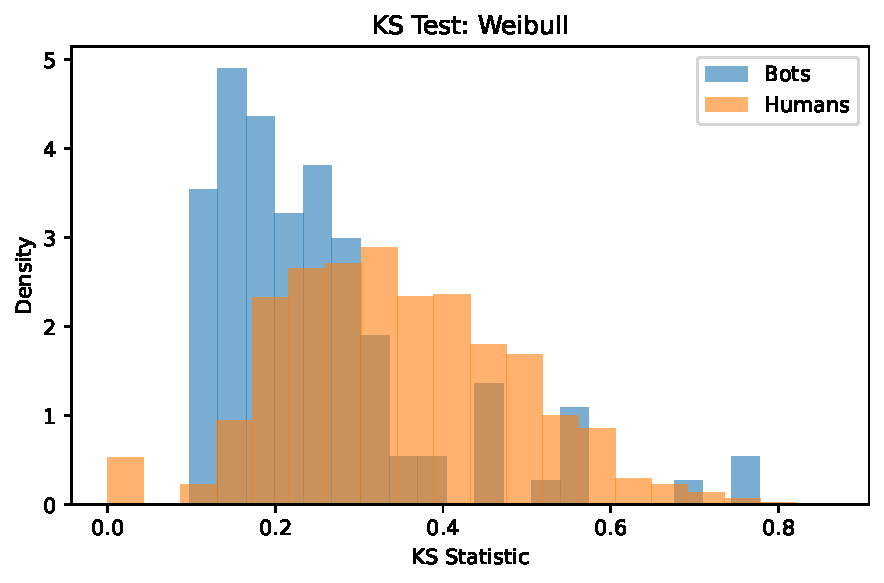
\includegraphics[width=\linewidth]{../figures/ks_weibull.pdf}
        \caption{Weibull model}
        \label{fig:ks_weibull}
    \end{subfigure}

    \caption{KS statistic distributions for inter-post intervals under various distributional fits.}
    \label{fig:ks_all_models}
\end{figure}

While a formal ablation study would be needed to 
confirm the hypothesis, the KS-based analysis supports our intuition that static temporal 
features are not reliable indicators of bot-like activity.
While the majority of bots fit the theoretical distributions more closely, 
the substantial overlap in KS statistics across all four models suggests
that these static summaries cannot capture the complex timing behaviors exhibited by sophisticated bots.

This finding, in part, motivates our shift toward deep multimodal architectures, 
where temporal information is represented in a more dynamic manner and learned jointly with other 
behavioral signals, enabling the model to uncover subtle, context-dependent 
patterns that handcrafted temporal features miss.


\subsection{Multimodal Architectures}

Recognizing the constraints of feature engineering, we
explored multimodal neural architectures directly modeling
sequences and cross-modal interactions inspired by recent
literature \textit{``Multimodal Detection of Bots on X (Twitter) using
Transformers''} \citep{ilias2023multimodal}, and \textit{``BotMoE: Twitter Bot Detection with Community-Aware
Mixtures of Modal-Specific Experts''} \citep{liu2023botmoe}. Our modalities include transformer-based
description and tweet embeddings alongside digital DNA representations (content and
temporal).

% This architectural shift draws inspiration from modern methods such as \textit{``Multimodal Detection of Bots on X (Twitter) using
% Transformers''} (Ilias et al., 2023), and \textit{``BotMoE: Twitter Bot Detection with Community-Aware
% Mixtures of Modal-Specific Experts''} (Liu et al., 2023). 

Evaluated architectures include:
\begin{itemize}
    \item \textbf{Gated Multimodal Unit (GMU)}: Dynamically weighting modalities.
    
    \item \textbf{Cross-Attention Fusion}: Learns cross-modal interactions through multihead attention.
    
    \item \textbf{Mixture-of-Experts (MOE)}: Subsets of the models specialize in different user types, with attention-based fusion and a learned convolution over attention weights.
\end{itemize}

These architectures not only provide greater modeling capacity, but also offer more robustness against feature manipulation, 
as they do not rely on manually crafted statistics. Instead, they operate directly over sequences of observed user behavior 
and learn to extract structure. 


\subsubsection{DNA Embedding Extraction}

To model user behavior beyond text embeddings, 
we construct symbolic sequences known as digital DNA, 
across the user's timeline chronologically,
representing content, timing, and emoji usage across tweets. 
These sequences are then converted into images and embedded 
via a CNN encoder. In all cases, the resulting character sequence 
is transformed into an image as follows:
\begin{enumerate}
    \item Each symbol is mapped to an 8-bit grayscale intensity value (e.g., \texttt{N} $\mapsto$ 0, \texttt{U} $\mapsto$ 64, ..., \texttt{X} $\mapsto$ 255).
    \item The sequence of grayscale values is reshaped into a square matrix: if the sequence has length $L$, the smallest $n \in \mathbb{N}$ such that $n^2 \geq L$ is selected. The sequence is zero-padded to length $n^2$ and reshaped to $(n \times n)$.
    \item This grayscale image is resized depending on the CNN encoder, using nearest-neighbor interpolation.
    \item The image is then converted to RGB format by replicating the grayscale channel, and the resulting
    tensor has shape: $3 \times \texttt{image\_width} \times \texttt{image\_height}$.
    \item The tensor is normalized using ImageNet statistics and passed through a pretrained CNN encoder. 
    % In our cross-attention
    % fusion methods, we used the MobileNetV2 encoder. We later found that MobileViT (small) yielded better performance and used it in the MOE appraoch. 
    \item The output features are either (1) average pooled and projected into a fixed embedding space, or (2) directly extracted from the last hidden layer of the CNN encoder.
\end{enumerate}

\textbf{Content DNA.} Each tweet is mapped to a symbol based on the type of entities it contains:
\begin{itemize}
    \item \texttt{N} --- No entities (plain text)
    \item \texttt{U} --- Contains a URL
    \item \texttt{H} --- Contains one or more hashtags
    \item \texttt{M} --- Contains one or more mentions
    \item \texttt{X} --- Contains a combination of multiple entity types
\end{itemize}

\textbf{Time DNA.}  
Time DNA encodes inter-post intervals by assigning symbols based on the time elapsed between consecutive tweets:
\begin{itemize}
    \item \texttt{n} --- First post (no delta)
    \item \texttt{o} --- $<$ 1 second
    \item \texttt{s} --- $\geq$ 1 second and $<$ 1 minute
    \item \texttt{m} --- $\geq$ 1 minute and $<$ 1 hour
    \item \texttt{h} --- $\geq$ 1 hour and $<$ 6 hours
    \item \texttt{u} --- $\geq$ 6 hours and $<$ 12 hours
    \item \texttt{x} --- $\geq$ 12 hours
\end{itemize}

\textbf{Emoji DNA.}  
We categorize emojis in tweets using a precompiled lookup table. Each tweet is assigned a category based on its emojis:
\begin{itemize}
    \item \texttt{S} — Smileys \& Emotion
    \item \texttt{P} — People \& Body
    \item \texttt{A} — Animals \& Nature
    \item \texttt{F} — Food \& Drink
    \item \texttt{T} — Travel \& Places
    \item \texttt{R} — Activities
    \item \texttt{O} — Objects
    \item \texttt{Y} — Symbols
    \item \texttt{L} — Flags
    \item \texttt{N} — No emoji present
    \item \texttt{X} — Multiple emoji categories
\end{itemize}

In all cases, these DNA images serve as behavioral \emph{fingerprints}, 
allowing CNNs to learn latent signals over them.



\subsubsection{Gated Multimodal Unit (GMU)}
The GMU allows the network to dynamically control how much 
each modality contributes to the final hidden representation.
The output is used (with possibly further transformation)
downstream for classification.

In the bimodal setting, where we consider two input modalities \( \mathbf{x}_v \) and \( \mathbf{x}_t \), 
the equations governing the GMU are as follows:
% the GMU computes separate intermediate representations \( \mathbf{h}_v \) and \( \mathbf{h}_t \) for each 
% modality using independent linear transformations followed by a nonlinearity. A sigmoid-based gating vector \( \mathbf{z} \) is then computed from the concatenated input and is used to weight the contribution of each modality to the final fused representation \( \mathbf{h} \).

\begin{align}
\mathbf{h}_v &= \tanh(\mathbf{W}_v \cdot \mathbf{x}_v) \\
\mathbf{h}_t &= \tanh(\mathbf{W}_t \cdot \mathbf{x}_t) \\
\mathbf{z} &= \sigma(\mathbf{W}_z \cdot [\mathbf{x}_v, \mathbf{x}_t]) \\
\mathbf{h} &= \mathbf{z} * \mathbf{h}_v + (1 - \mathbf{z}) * \mathbf{h}_t \\
\mathbf{\Theta} &= \{ \mathbf{W}_v, \mathbf{W}_t, \mathbf{W}_z \} 
\end{align}

Here, \( \mathbf{h}_v \) and \( \mathbf{h}_t \) are hidden states learned on modalities \( \mathbf{x}_v \) and \( \mathbf{x}_t \),
\([\mathbf{.} , \mathbf{.}] \) denotes concatenation, and \(\mathbf{\Theta} \) denotes learnable parameters.
Cross-modal interactions are learned in the parameters \( \mathbf{W}_z\), 
the weighting mechanism \(\mathbf{z} \)
then applies a sigmoid activation \(\sigma \) on the projected modalities
to determine how much each one contributes to the final fused representation.
In practice, implementations tend to depart\footnote{ \citet{arevalo2017gated}’s own demo \url{https://github.com/johnarevalo/gmu-mmimdb/blob/master/model.py}; omits separate projections for each modality and applies the nonlinearity directly to the inputs.}
from some of the original equations,
including ours.

% \footnote{The hidden states were concatenated for weighting, 
% which improved training stability.}.



Resembling the work of \citet{ilias2023multimodal}, our intial efforts with the GMU used the following modalities:
\begin{itemize}
    \item User description embedding from TwHIN-BERT.
    \item Content-DNA embedding from MobileNetV2.
\end{itemize}
The first iteration consisted of a two layer classification head applied
to the GMU's output. This model marked all samples as negatives,
and several adjustments were needed. Working backwards from 
our final iteration, we reason that the first attempt 
was ineffective because it did not use normalization to deal with input variation and was unable to learn cross-modal interactions effectly due to its simple linear gating mechanism.

\paragraph{Architectural Progression Toward the Final GMU.}
To improve the initial GMU, we developed refined variants with the following changes:

\begin{itemize}
    \item Introduced modality-specific projections and \textit{LayerNorm} to balance their scales. 
    Normalization was applied after fusion to stabilize the representation.

    \item Added a global residual connection that projected modality embeddings directly to the hidden space, and applied modality-specific dropout.
\end{itemize}

\paragraph{Incorporating Time-DNA and Its Impact.}
While refining our GMUs, time-DNA embeddings were introduced as a third modality.
Despite content- and time-DNA representing the same modality, this addition improved performance, 
supporting our intuition that a dynamic temporal feature can help capture richer distinctions 
between bots and humans.

While our GMU iterations demonstrated nontrivial improvements, 
development required numerous adjustments to stabilize training 
and optimize performance. 
This raised concerns about generalizability;
would such a carefully balanced architecture transfer 
effectively to different modalities and datasets?

Given these concerns, we transitioned to a cross-modal attention approach, 
expecting that it could acheive nontrivial performance with fewer 
architectural tweaks.


\subsubsection{Cross-Attention}
We first learn an intermediate representation of the DNA embeddings (content and time)
to later apply cross-attention with the user description. We found that employing
a GMU to learn a fused DNA representation was effective, despite its intended multimodal use.

Our cross-attention method fuses text (user description) and DNA in the following way:
\begin{itemize}
    \item Apply a simple GMU to the DNA embeddings to create an intermediate representation 
    of fused-DNA.
    \item Apply cross-attention layers to the description and fused-DNA in both directions.
\end{itemize}

To perform cross-modal attention, we employ two multihead-attention layers,
computing scaled dot-product attention \citep{vaswani2017attention}
\begin{align}
    \text{Attention}(Q, K, V) &= \text{softmax}(\frac{QK^{T}}{\sqrt{d_k}})V
\end{align}
in one direction where the description modality is the query (Q) and fused-DNA 
provides the key (K) and value (V), and another direction in which the modalities swap 
roles. Here, $d_k$ denotes the dimensionality of the query and key. 
A mean pooling is then applied to attention outputs to form 
a final fused representation.

With the fused representation, we began with a 
two layer classification head and iteratively improved our architecture.
This required less refinements than our GMU approach. 

\paragraph{Sessions 16-17 - Description, Content, Time}
For session 16, we employed the cross-attention approach
on user description embeddings and CNN-encoded content 
and time DNA sequences.

\textbf{Architecture:} Along with the previously outlined steps, 
The design follows a structured flow employing conventional 
methods such as residual connections and layer normalization:
\begin{itemize}
    \item \textbf{Cross-Modal Fusion:}
    \begin{itemize}
        \item \textbf{Pre-Layer normalization} \citep{xiong2020layer} and \textbf{residual connections} are applied at each attention stage to stabilize training and preserve modality-specific signals.
    \end{itemize}
    
    \item \textbf{Feature Refinement:}
    \begin{itemize}
        \item The two cross‑attention outputs are concatenated into a tiny sequence and fed through a single position‑wise FFN, 
        enabling direct interaction between modalities while sharing parameters for better regularization.
        \item A residual connection around the FFN plus a preceding LayerNorm ensure stable feature propagation and consistent scaling.
    \end{itemize}
    
    \item \textbf{Aggregation and Prediction:}
    \begin{itemize}
        \item \textbf{Global average pooling} condenses the multi-token output into a single fused vector.
        \item A \textbf{two-layer classification head} generates the final logits for bot detection.
    \end{itemize}
\end{itemize}

\textbf{Strengths:}
\begin{itemize}
  \item \textit{Hierarchical fusion}: In addition to the bidirectional cross‑attention steps, GMU’s gated combination of content and time embeddings produces richer joint representations than simple concatenation alone.
%   \item \textit{High expressiveness}: Beyond the cross‑attention fusion, treating each modality as its own token and then merging them enables the model to capture subtle behavioral cues (e.g., burst patterns or nuanced profile signals) that flatter architectures miss.
\end{itemize}

\textbf{Weaknesses:}
\begin{itemize}
  \item \textit{Overparameterization risk}: Multiple attention layers plus gating mechanisms add significant complexity, making the model prone to overfitting without sufficient data or strong regularization.
  \item \textit{Hyperparameter sensitivity}: Stable training depends on careful tuning of learning rate, dropout rate, number of heads, gating biases, etc.; suboptimal settings can lead to slow convergence or degraded performance.
\end{itemize}

\textbf{Performance:} The model underperformed relative to some of our random forest attempts. However, the bots had improved significantly by session 16, 
and a drop in performance was expected given the model's complexity and the limited fine-tuning conducted at this stage.

\textbf{Conclusion:} While the session 16 model introduced a promising fusion paradigm combining gated mechanisms and cross-modal attention, 
it fell short in performance due to its tuning demands. 
Nonetheless, this model performed well given its complexity and lack of tuning, and it set the stage for our future attempts.


\paragraph{Sessions 18-19 - Description, Content, Time, Emoji}
For sessions 18 and 19, the model remained the same, 
except that we extended the GMU to fuse 
three DNA embeddings: content, time, and emoji. Our intuition was that
LLM-powered bots exhibit obvious tells in their use of emojis across posts.

\textbf{Weaknesses and Challenges}:
\begin{itemize}
    \item \textit{Marginal Utility of Emoji Features:} Despite their inclusion, the emoji embeddings did not noticeably improve performance. Their sparse and high-dimensional nature may have diluted their utility. 
    Future work could explore reducing the emoji vocabulary and using lower-dimensional embeddings to better leverage these signals.
    \item \textit{Training Instability:} Adding a third modality introduced some training instability, as the model exhibited greater sensitivity to hyperparameter configurations.
    \item \textit{Overparameterization Risk:} As in previous sessions, the model remains sensitive to overfitting due to its multiple attention layers and gating mechanisms.
\end{itemize}

\textbf{Performance:} Overall, the inclusion of emoji DNA and the extended GMU yielded only marginal performance changes compared to previous attempts. 
While feature expressiveness theoretically increased, training instability and limited emoji utility constrained practical improvements.

\textbf{Conclusion:} Sessions 18 and 19 served to explore the feasibility of extending 
our fusion mechanism to include emoji signals. The experiment revealed the challenges 
of integrating sparse representations like emojis. Future refinements may involve dimensionality 
reduction or selective filtering of emoji types to enhance their contribution.

Although a cross-attention approach can be effective,
it is computationally expensive to scale
beyond two modalities. For example, three modalities would 
require six multihead-attention layers to consider 
each cross-modal interaction in both directions.

A natural alternative is to employ a single self-attention 
block where each token corresponds to a modality. 
A key challenge in this approach is learning modality representations to provide to
the self-attention layer. 
We find that MOEs learn these representations effectively, and in particular, 
are better at modelling the diverse user behaviours found on X.


\subsubsection{Mixture-of-Experts (MoE)}
To address the challenges of (1) model scalability and (2) diverse bot behaviors 
across user communities, we closely follow the \textbf{Mixture-of-Experts (MoE)} 
strategy employed by \citet{liu2023botmoe}. This approach leverages specialized 
experts conditioned on user sub-communities, enabling community-aware representation learning.

% Noting that user descriptions can be easily manipulated, we also
% sample five tweets from the user, uniformly across their timeline.


\paragraph{Expert Assignment and Gating}
For each modality (text, DNA), user embeddings are fed into a \textbf{gating network}:
\begin{align}
G(\mathbf{x}) &= \text{softmax}(\text{KeepTopK}(W_g \mathbf{x}, k))
\end{align}
where \( W_g \) are learnable weights, \( \mathbf{x} \) is the input embedding, and \texttt{KeepTopK} retains the top \( k \) gating scores for sparse expert activation.

\paragraph{Expert Aggregation}
The final representation for modality \( m \in \{t=\text{text}, d=\text{DNA}\} \) is a weighted sum of expert outputs:
\begin{align}
\mathbf{z}_i^{(m)} &= \sum_{j=1}^{n} G(\mathbf{x}_i^{(m)})_j E_j(\mathbf{x}_i^{(m)})
\end{align}
where \( E_j(\cdot) \) denotes the \( j^\text{th} \) expert (a two-layer MLP), and \( G(\mathbf{x}_i^{(m)})_j \) is the gating score for expert \( j \).

\paragraph{Feature Fusion and Consistency}
After expert aggregation, representations across modalities are fused using a \textbf{multi-head self-attention} mechanism:
\begin{align}
\{\tilde{\mathbf{z}}^{(t)}, \tilde{\mathbf{z}}^{(d)}\} &= \text{SelfAttn}(\{\mathbf{z}^{(t)}, \mathbf{z}^{(d)}\})
\end{align}
Additionally, we compute a \textbf{consistency matrix} between the modalities and downsample it:
\begin{align}
\mathbf{z}^{(con)} &= \text{flatten}(\text{Conv2D}(\text{sample}(\mathbf{M})))
\end{align}
where \( \mathbf{M} \) is the attention matrix across modalities, and the convolution extracts cross-modal consistency signals.

\paragraph{Classification Head}
The fused representations and consistency vector are concatenated and passed through a final classifier:
\begin{align}
y_i &= W_o \cdot [\tilde{\mathbf{z}}^{(t)}, \tilde{\mathbf{z}}^{(d)}, \mathbf{z}^{(con)}] + b_o
\end{align}
where \( W_o \) and \( b_o \) are learnable parameters.

\paragraph{Loss Function:}
We optimize a \textbf{cross-entropy loss} with two regularization terms:
\begin{align}
\mathcal{L} &= -\sum_{i \in \mathcal{Y}} t_i \log y_i + \lambda_1 \sum_{\theta} \|\theta\|_2^2 + \lambda_2 \sum_{i \in \mathcal{Y}} \sum_{m \in \{t, d\}} BL(\mathbf{x}_i^{(m)})
\end{align}
where \(\theta \) denotes model parameters (that is, we use L2-regularization) and \( BL(\cdot) \) is the \textbf{balancing loss} from \citet{shazeer2017outrageously}:
\begin{align}
BL(\mathbf{x}) &= w_{imp} \cdot CV(G(\mathbf{x}))^2 + w_{ld} \cdot CV(P(\mathbf{x}, i))^2
\end{align}
Here, \( CV \) is the coefficient of variation, encouraging balanced expert usage.

\paragraph{Sessions 20-21 - Text, DNA}
For sessions 20 and 21, we incorporated the MoE architecture to replace earlier cross-attention mechanisms. Each modality (text and DNA) is processed by its respective \textbf{community-aware MoE} layer.

\textbf{Architecture:}
\begin{itemize}
    \item \textbf{Modality-specific Experts:} Each modality employs two to three experts, activated via sparse gating to promote community-aware specialization.
    \item \textbf{Fusion and Consistency:} Outputs from experts are fused via multi-head self-attention, with cross-modal consistency extracted via convolutional filters over attention matrices.
    \item \textbf{Prediction:} The fused and consistent representations are passed through a two-layer classification head.
\end{itemize}

\textbf{Strengths:}
\begin{itemize}
    \item \textit{Efficiency}: It is the smallest of our multimodal models, requiring less time to train and perform inference.
    \item \textit{Community-aware specialization}: Each expert learns patterns within specific user sub-communities, improving generalization across diverse bot behaviors.
    \item \textit{Balanced expert utilization}: The balancing loss encourages fair expert usage, preventing mode collapse and overfitting.
\end{itemize}

\textbf{Challenges:}
\begin{itemize}
    % \item \textit{Computational overhead:} The gating mechanism and expert selection introduce extra computation, especially when scaling to more modalities or larger datasets.
    \item \textit{Hyperparameter tuning:} Similar to our cross-attention models, MoE layers exhibit sensitivity to hyperparameters like expert count and gating sparsity.
\end{itemize}

\textbf{Performance:} Despite the increased model complexity, MoE-based models exhibited better generalization across communities but did not significantly outperform simpler baselines due to limited training time.

\textbf{Conclusion:} The MoE framework effectively captured community-specific bot behaviors and offered a scalable alternative to cross-attention fusion, though further tuning and expert design could improve stability and performance.







\section{Discussion}
blah blah....

\section{Conclusion and Future Work}
blah blah...

% \bibliographystyle{IEEEtran}
\bibliographystyle{plainnat}
\bibliography{references}






\end{document}